% ---- Document Class ----
\documentclass[sn-mathphys,Numbered]{sn-jnl}

% ---- Essential Packages ----
% FIX: Load xcolor ONCE with all necessary options to prevent "Option Clash"
\usepackage[table,dvipsnames,svgnames]{xcolor}

\usepackage{amsmath}
% FIX: Handle \Bbbk conflict before loading amssymb
\let\Bbbk\relax 
\usepackage{amssymb}
\usepackage{mathtools}
\usepackage{amsthm}

\usepackage[demo]{graphicx} % 'demo' allows compiling without images
\usepackage{hyperref}

% ---- Formatting & Layout ----
\usepackage{alltt}
\usepackage{paralist}
\usepackage{booktabs}
\usepackage{multirow}
\usepackage{arydshln}
\usepackage{wrapfig}
\usepackage[export]{adjustbox}
\usepackage{enumitem}
\usepackage{float}
\usepackage{caption}
\usepackage{subcaption}
\usepackage{tcolorbox}
\usepackage{nicefrac}

% ---- Code Listings ----
\usepackage{listings}
\usepackage{verbatim}

% ---- Math & Symbols ----
\usepackage{mathpartir}
\usepackage{wasysym}
\usepackage{pifont}
\usepackage{stmaryrd}
\usepackage{bussproofs}
\usepackage{gensymb}
\usepackage[per-mode=symbol,detect-all]{siunitx}

% ---- Other Utilities ----
\usepackage{xspace}
\usepackage{url}
\usepackage{svg}
\usepackage{ifthen}
\usepackage{etoolbox}
\usepackage[outline]{contour}

% ---- TikZ Graphics ----
\usepackage{tikz}
\usetikzlibrary{shapes.geometric,positioning,arrows}

% ---- Cleveref (Must be loaded after hyperref) ----
\usepackage[capitalize]{cleveref}

% ---- Custom Definitions & Macros ----

% Theorem environments
\newtheorem{theorem}{Theorem}[section]
\newtheorem{lemma}[theorem]{Lemma}
\newtheorem{proposition}[theorem]{Proposition}
\newtheorem{corollary}[theorem]{Corollary}
\theoremstyle{definition}
\newtheorem{definition}[theorem]{Definition}
\theoremstyle{remark}
\newtheorem{remark}[theorem]{Remark}

% Colors
\definecolor{brightyellow}{RGB}{255,247,192}
\definecolor{lightchacki}{RGB}{245,237,205}
\definecolor{darkorange}{RGB}{255,140,0}
\definecolor{headerbg}{RGB}{220,230,241}

% Symbols
\newcommand{\cmark}{\checkmark}
\newcommand{\xmark}{\textcolor{red}{\ding{55}}}
\newcommand{\greencmark}{\textcolor{green}{\ding{51}}}

% Math Macros
\newcommand{\cfg}[3]{\langle #1,\; #2,\; #3\rangle}
\newcommand{\update}[3]{#1[#2 \mapsto #3]}
\newcommand{\step}{\mathrel{\rightarrow}}
\newcommand{\pstep}{\mathrel{\Rightarrow}}
\newcommand{\Pre}{\mathsf{pre}}
\newcommand{\Post}{\mathsf{post}}
\newcommand{\toolname}{\textsc{Ser}}
\newcommand{\grammartag}[1]{\qquad\qquad\emph{(#1)}}

% Keywords
\newcommand{\kw}[1]{\textbf{#1}}
\newcommand{\nondet}{\kw{?}}
\newcommand{\ifkw}{\kw{if}}
\newcommand{\elsekw}{\kw{else}}
\newcommand{\whilekw}{\kw{while}}
\newcommand{\yieldkw}{\kw{yield}}
\newcommand{\requestkw}{\kw{request}}
\newcommand{\sat}{\texttt{SAT}}
\newcommand{\unsat}{\texttt{UNSAT}}
\newcommand{\Parikh}{\mathsf{Parikh}}

% Helper commands
\newcommand\blfootnote[1]{%
	\begingroup
	\renewcommand\thefootnote{}\footnote{#1}%
	\addtocounter{footnote}{-1}%
	\endgroup
}

\newcommand{\guy}[1]{\marginpar{\textcolor{orange}{Guy: #1}}}
\newcommand{\jules}[1]{\marginpar{\textcolor{red}{Jules: #1}}}
\newcommand{\markb}[1]{\marginpar{\textcolor{black}{Mark: #1}}}
\newcommand{\todo}[1]{\textcolor{red}{TODO: #1}}

% Listings Configuration
\lstdefinelanguage{CustomPseudoCode}{
	morekeywords={request, yield, return, if, else, while, and, or},
	morecomment=[l]{//},
	morestring=[b]",
	sensitive=true
}

\lstset{
	language=CustomPseudoCode,
	basicstyle=\ttfamily\small,
	keywordstyle=\color{blue}\bfseries,
	commentstyle=\color{gray}\itshape,
	stringstyle=\color{orange},
	numbers=left,
	numberstyle=\tiny,
	stepnumber=1,
	numbersep=5pt,
	backgroundcolor=\color{white},
	frame=single,
	rulecolor=\color{black},
	tabsize=2,
	captionpos=b,
	breaklines=true,
	breakatwhitespace=false,
	showstringspaces=false,
	escapeinside={(*@}{@*)},
}

% Hyperref fixes
\makeatletter
\renewcommand*{\theHsection}{\thesection}
\renewcommand*{\theHsubsection}{\thesubsection}
\renewcommand*{\theHsubsubsection}{\thesubsubsection}
\patchcmd{\@sect}
{\@tempskipa #5\relax}
{\refstepcounter{#1}%
	\Hy@raisedlink{\hyper@anchorstart{#1.\csname the#1\endcsname}\hyper@anchorend}%
	\@tempskipa #5\relax}
{}{}
\makeatother

% ==========================================
%            DOCUMENT START
% ==========================================
\begin{document}
	
	\title{Deciding Serializability in Network Systems}
	
	\author*[1]{\fnm{Guy}\sur{Amir}}\email{gda42@cornell.edu}
	\author[1]{\fnm{Mark}\sur{Barbone}}\email{mlb494@cornell.edu}
	\author[2]{\fnm{Nicolas}\sur{Amat}}\email{nicolas.amat@onera.fr}
	\author[1]{\fnm{Jules}\sur{Jacobs}}\email{jj758@cornell.edu}
	
	\affil[1]{\orgname{Cornell University}, \orgaddress{\city{Ithaca}, \country{United States}}}
	\affil[2]{\orgname{DTIS, ONERA, Universit\'e de Toulouse}, \orgaddress{\city{Toulouse}, \country{France}}}
	
	\abstract{
		We present the \toolname{} modeling language for automatically verifying \textit{serializability} of concurrent programs.
		\toolname{} programs are suitably restricted to make this problem decidable, while still allowing for an \textit{unbounded} number of concurrent threads.
		
	}
	
	\keywords{Serializability, Concurrent programs, Network systems, Petri nets, Decision procedure}
	
	\maketitle
	\pagestyle{plain}
	\thispagestyle{plain}
	
	% PLACEHOLDERS FOR CONTENT
	% (Uncomment your \input lines when running locally)
	
	\section{Introduction}
	% \section{Introduction}
\label{sec:introduction}

\todo{Introduction goes here.}

\todo{We motivate the problem of deciding serializability in programmable networks.}

\todo{We talk about some related work if relevant.}

\todo{We show that it's interesting with an example.}

\todo{We describe our main results.}

\paragraph{Contributions:}
\begin{itemize}
    \item Novel notion of serializability (``atomicity'') applicable to network systems
    \item Decidability results (1 main theorem: \textbf{automatically proving unbounded serializability}, 2 extra theorems: ser=ser decidable, ser=int undecidable)
    \item Implementation of decision procedure
    \item Advances in semilinear sets, Petri net reachability heuristics that makes the decision procedure work
\end{itemize}
	This is placeholder text for the introduction.
	
	\section{Problem Definition}
	% \section{Problem Definition}
\label{sec:problemDefinition}

\begin{figure}[t]
    \begin{align*}
    e ::= &&&\\
       | & \; 0 \mid 1 \mid 2 \mid \ldots                                && \text{(numeric constants)} \\
       | & \; \nondet                                 && \text{(nondeterministic value: 0 or 1)}\\
       | & \; x := e                            && \text{(write to local variable / packet field)} \\
       | & \; x                                 && \text{(read from local variable / packet field)} \\
       | & \; X := e                            && \text{(write to global variable / switch variable)} \\
       | & \; X                                 && \text{(read from global variable / switch variable)} \\
       | & \; e_1 == e_2                        && \text{(equality test)} \\
       | & \; e_1 ; e_2                         && \text{(sequencing)} \\
       | & \; \ifkw(e_1)\{e_2\}\elsekw\{e_3\} && \text{(conditional)} \\
       | & \; \whilekw(e_1)\{e_2\}              && \text{(loop)} \\
       | & \; \yieldkw                      && \text{(yields to scheduler)}
    \end{align*}
    \caption{Syntax of expressions}
    \label{fig:syntax}
\end{figure}
    
A Network System $\mathcal{N}$ is a tuple $(G, L, \mathit{Req}, \mathit{Res}, g_0, \delta, \mathit{req}, \mathit{resp})$ where:
\begin{itemize}
\item $G$ is a set of global states representing switch state
\item $L$ is a set of local states representing packet contents
\item $\mathit{Req}$ is a set of request events
\item $\mathit{Res}$ is a set of response events
\item $g_0 \in G$ is the initial global state
\item $\mathit{req} \subseteq \mathit{Req} \times L$ is a request transition relation, which describes which requests turn into which packets
\item $\mathit{resp} \subseteq L \times \mathit{Res}$ is a response transition relation, which describes which packets turn into which responses
\item $\delta \subseteq (G \times L) \times (G \times L)$ is a transition relation for packet processing, which describes an atomic step of packet processing that may change the global state.
\end{itemize}

\begin{figure}[t]
    \centering
    \renewcommand{\arraystretch}{1.6}
    \[
    \begin{array}{c}
    \textbf{States and Transitions:}
    \\
    \quad
    \text{A (global) \emph{network state} is a triple }(g,\mathcal{P},M)\text{ where:}
    \\
    \quad
    g \in G \text{ is the current global switch state,}
    \\
    \quad
    \mathcal{P} \in \text{Multiset}(L \times \mathit{Req}) \text{ is a multiset of in-flight packets,}
    \\
    \quad
    M \in \text{Multiset}(\mathit{Req} \times \mathit{Res}) \text{ is a multiset of request--response pairs already completed.}
    \end{array}
    \]

    \[
    \begin{array}{c}
    \textbf{Initial state:}
    \\
    \quad (g_0,\,\varnothing,\,\varnothing)
    \end{array}
    \]

    \[
    \begin{array}{c}
    \textbf{Transition rules:}
    \\[1em]
    \text{(New Request)}\quad\infer{
    (r,\ell)\,\in\,\mathit{req}
    }
    {(g,\;\mathcal{P},\;M) \;\longrightarrow\; (g,\;\mathcal{P} \uplus \{(\ell,r)\},\;M)}
    \\[2em]
    \text{(Packet Step)}\quad\infer{
    ((g,\ell),\,(g',\ell')) \,\in\, \delta
    }
    {(g,\;\mathcal{P} \uplus \{(\ell,r)\},\;M) \;\longrightarrow\; (g',\;\mathcal{P} \uplus \{(\ell',r)\},\;M)}
    \\[2em]
    \text{(Response)}\quad\infer{
    (\ell,s)\,\in\,\mathit{resp}
    }
    {(g,\;\mathcal{P} \uplus \{(\ell,r)\},\;M) \;\longrightarrow\; (g,\;\mathcal{P},\;M \uplus \{(r,s)\})}
    \end{array}
    \]

    \[
    \begin{array}{c}
    \textbf{Complete runs:}
    \\
    \quad (g_0,\,\varnothing,\,\varnothing) \;\longrightarrow\; (g_1,\,\mathcal{P}_1,\,M_1) \;\longrightarrow\; \cdots \;\longrightarrow\; (g_n,\,\mathcal{P}_{n-1},\,M_{n-1}) \;\longrightarrow\; (g_n,\,\varnothing,\,M_n)
    \\[1em]
    \textbf{Interleaved run: } \text{the } \mathcal{P}_i \text{ can have more than one packet, and } \mathcal{P}_n = \varnothing \\
    \textbf{Serial run: } \text{ each } \mathcal{P}_i \text{ has at most one packet, and } \mathcal{P}_n = \varnothing\\
    \text{Int}(\mathcal{N}) = \{ M \in \text{Multiset}(\mathit{Req} \times \mathit{Res}) \mid \exists \text{ interleaved run } (g_0,\,\varnothing,\,\varnothing) \;\longrightarrow^*\; (g_n,\,\varnothing,\,M) \}\\
    \text{Ser}(\mathcal{N}) = \{ M \in \text{Multiset}(\mathit{Req} \times \mathit{Res}) \mid \exists \text{ serial run } (g_0,\,\varnothing,\,\varnothing) \;\longrightarrow^*\; (g_n,\,\varnothing,\,M) \}\\
    \end{array}
    \]

    \caption{State-transition rules for executions of
    \(\mathcal{N} = (G, L, \mathit{Req}, \mathit{Res}, g_0, \delta, \mathit{req}, \mathit{resp})\).
    A transition \(\longrightarrow\) modifies the triple \((g,\mathcal{P},M)\) by either (1) introducing a new request, (2) processing a packet step via \(\delta\), or (3) consuming a packet to produce its response.  When no more steps are possible, the result set \(M\) is the final multiset of request--response pairs that arose during the run.
    Runs are called \emph{serial} if there is at most one packet in flight at any time, whereas \emph{interleaved} runs may have multiple packets in flight at once.}
    \label{fig:network-transitions}
\end{figure}

\begin{definition}[Interleaved executions \(\mathrm{Int}(\mathcal{N})\)]
    Let \(\mathcal{N} = (G, L, \mathit{Req}, \mathit{Res}, g_0, \delta, \mathit{req}, \mathit{resp})\).
    An \emph{interleaved execution} begins in global state \(g = g_0\) with no packets in flight.
    At any point, one may:
    \begin{itemize}
        \item introduce a new request \(r \in \mathit{Req}\), producing an in-flight packet \(\ell \in L\) if \((r,\ell) \in \mathit{req}\);
        \item take an in-flight packet \(\ell\) and transition \(\ell \mapsto \ell'\) and \(g \mapsto g'\) if \(((g,\ell),(g',\ell'))\in\delta\);
        \item consume an in-flight packet \(\ell\) to produce a response \(s\) if \((\ell,s)\in \mathit{resp}\).
    \end{itemize}
    Each request \(r\) must eventually yield exactly one corresponding response \(s\) in a valid execution.
    The set of all finite multisets of \((r,s)\) pairs realizable by such interleavings is:
    \[
        \mathrm{Int}(\mathcal{N})
        \;=\;
        \bigl\{
        M \;\in\; \text{Multiset}(\mathit{Req}\times \mathit{Res})
        \;\mid\;
        M \text{ is realized by some interleaved run of }\mathcal{N}
        \bigr\}.
    \]
\end{definition}

\begin{definition}[Serial executions \(\mathrm{Ser}(\mathcal{N})\)]
In a \emph{serial} execution, requests are processed one at a time:
\begin{enumerate}
    \item Start in \(\,g_0\).
    \item Take a single request \(r\in \mathit{Req}\), convert it to a packet, process that packet until a response \(s\in \mathit{Res}\) is produced.
    \item Update the global state accordingly and repeat with the next request.
\end{enumerate}
No two requests overlap in processing.
The set of all finite multisets of \((r,s)\) pairs realizable by such one-at-a-time runs is:
\[
    \mathrm{Ser}(\mathcal{N})
    \;=\;
    \bigl\{
    M \;\in\; \text{Multiset}(\mathit{Req}\times \mathit{Res})
    \;\mid\;
    M \text{ is realized by some serial run of }\mathcal{N}
    \bigr\}.
\]
\end{definition}

\begin{theorem}[Serializability]
\label{thm:int-eq-ser}
Whether
\(
    \mathrm{Int}(\mathcal{N}) \;=\; \mathrm{Ser}(\mathcal{N})
\)
holds is decidable.
\end{theorem}

\begin{theorem}[Serial Equivalence]
\label{thm:ser-eq-ser}
Whether
\(
    \mathrm{Ser}(\mathcal{N}) \;=\; \mathrm{Ser}(\mathcal{N})
\)
holds is decidable.
\end{theorem}

\begin{theorem}[Interleaved Equivalence]
\label{thm:int-eq-int}
Whether
\(
    \mathrm{Int}(\mathcal{N}) \;=\; \mathrm{Int}(\mathcal{N})
\)
holds is undecidable.
\end{theorem}
	This is placeholder text for the problem definition.
	
	
	\section{Formal Results}
	% \section{Formal results}
\label{sec:formal-results}

	This is placeholder text for formal results.
	
	\section{Implementation}
	% 

\section{Implementation}
\label{sec:implementation}
\begin{wraptable}[11]{r}{0.32\textwidth}
	\vspace{-1.5em} 
	\centering
	\begin{tabular}{@{} l S[table-format=5.0] @{}}
		\toprule
		\textbf{Module}                & {\textbf{LoC}} \\
		\midrule
		Input \& Parsing               &  1723          \\
		Model Construction             &  5561          \\
		Petri--Net Conversion           &   843          \\
		Reachability          &  2628          \\
		Proof Checking                 &  3240          \\
		Utilities                      &  2160          \\
		Testing \& Evaluation          &  2118          \\
		\midrule
		\textbf{Total}                 & \textbf{18273} \\
		\bottomrule
	\end{tabular}
	\caption{Lines of Code}
	\label{tab:loc_summary2}
\end{wraptable}
%\vspace{-1.5\baselineskip} % nudge following text up a bit
We implemented our approach in \toolname{}~\cite{ArtifactRepository}, a publicly available toolchain consisting of over $18{,}200$ LoC written mostly in \texttt{Rust} (see Table~\ref{tab:loc_summary2}).
%
%We next elaborate on the architecture of our tool and the various optimizations we added to allow it to run efficiently.
%
%For the underlying Petri Net model checker, we use SMPT~\cite{AmDa23} which supports \textit{unbounded} reachability queries (see Appendix~\ref{appendix:smpt}).
%, and which uses Z3 as an underlying SMT solver~\cite{DeBj08}. 
%and which we extended to support our setting (for example, we needed to extend the solver to support proof generation). 
%
%We note that other off-the-shelf solvers can be used as well.

%The implementation..

%\begin{enumerate}
%	\item The extra things we did to make the thing actually run
%	\item Code architecture
%	\item Optimizations
%\end{enumerate}

%\newpage
\subsection{Code Architecture}

%\begin{tabular}{|l|r|}
%	\hline
%	\textbf{Module} & \textbf{LoC} \\
%	\hline
%	Input \& Parsing                             & 1723  \\
%	\hline
%	Model Construction                           & 5561  \\
%	\hline
%	Petri-Net Conversion                         & 843   \\
%	\hline
%	Reachability Checking                        & 2628  \\
%	\hline
%	Proof Checking                               & 3240  \\
%	\hline
%	Utilities                                       & 2160  \\
%	\hline
%	Testing \& Evaluation               & 2118  \\
%	\hline
%	\textbf{Total}                               & \textbf{18273} \\
%	\hline
%\end{tabular}


%
%\begin{table}[ht]
%	\centering
%	\label{tab:loc_summary}
%	\begin{tabular}{@{} l S[table-format=5.0] @{}}
%		\toprule
%		\textbf{Module}                & {\textbf{LoC}} \\
%		\midrule
%		Input \& Parsing               &  1723          \\
%		Model Construction             &  5561          \\
%		Petri–Net Conversion           &   843          \\
%		Reachability Checking          &  2628          \\
%		Proof Checking                 &  3240          \\
%		Utilities                      &  2160          \\
%		Testing \& Evaluation          &  2118          \\
%		\midrule
%		\textbf{Total}                 & \textbf{18273}          \\
%		\bottomrule
%	\end{tabular}
%	\caption{Lines of Code by Module}
%\end{table}
%

% Then, where you want the table wrapped to the right:
%
% this table summarizes the values without whitespaces/comments and without the code for SMPT (or the wrapper) or the carfo and toml files
%
%\begin{wraptable}[8]{r}{0.32\textwidth}
%	\centering
%	\begin{tabular}{@{} l S[table-format=5.0] @{}}
%		\toprule
%		\textbf{Module}                & {\textbf{LoC}} \\
%		\midrule
%		Input \& Parsing               &  1723          \\
%		Model Construction             &  5561          \\
%		Petri–Net Conversion           &   843          \\
%		Reachability          &  2628          \\
%		Proof Checking                 &  3240          \\
%		Utilities                      &  2160          \\
%		Testing \& Evaluation          &  2118          \\
%		\midrule
%		\textbf{Total}                 & \textbf{18273} \\
%		\bottomrule
%	\end{tabular}
%	\caption{Lines of Code (LoC)}
%	\label{tab:loc_summary2}
%\end{wraptable}
%
%\noindent
%
\toolname{} implements an end-to-end serializability checker for a given input program. If the program is serializable, we return a proof thereof; otherwise, if it is not serializable, a counterexample is given to the user for an interleaving that can result in request/response pairs that are unattainable in any serial execution.
%
Our workflow translates the decidability problem to an equivalent Petri net reachability question (for an unbounded number of tokens), in which (i) the Petri net represents all possible interleavings of the program; and (ii) the reachability query represents a semilinear set (equivalently, a Presburger arithmetic encoding) of all request/response pairs that \textit{cannot} be obtained by any serial execution.
%
As Petri net reachability is \texttt{Ackermann}-complete~\cite{CzWo22}, we added various optimizations to expedite the search process, both at the PN level and the property-encoding level.
%
The pipeline of \toolname{} is depicted in Fig.~\ref{fig:full_program_flow}, and includes:
 

\begin{enumerate}
	\item \textbf{Input \& parsing.} 
	Our framework receives either a \texttt{SER} program with the syntax described in~\Cref{sec:problem-definition}; or a \texttt{JSON} file directly encoding a network system. In the case of the former, an additional step takes place, parsing the input %(using the \texttt{parser.rs} module) 
	to an expression tree that is translated to the equivalent NS.
%	, represented as a struct in the \texttt{ns.rs} module. 
	
	\item \textbf{Petri net conversion.} The NS is then translated into a Petri net 
%	(see the \texttt{petri.rs} module) 
which represents all possible interleavings. 
%	.as depicted, for example, in subsec.~\ref{subsec:ns-not-serializable}.
%	Each place represents a state (either global or local) or a response. Each token represents a single in-flight request or a terminated response. 
The PN is encoded in the de facto standard \texttt{NET} format, to support off-the-shelf PN model checkers. 
	
	\item \textbf{Semilinear conversion.} 
%	This includes a set of modules (\texttt{kleene.rs}, \texttt{semilinear.rs}, and \texttt{presburger.rs}) which 
We generate a semilinear set encoding all non-serializable outputs, via translation of the serialized NFA (e.g., Fig.~\ref{fig:code2ExampleNFA}) to a regex, which is then projected (via the Parikh image) and complemented. 
%	This conversion is done by the following pipeline: (1) the NS is translated to an NFA encoding all possible request/response pairs of the input program; (2) This NFA is translated to a regex (via Kleene's Theorem) and then projected (via the Parikh Image) to a semilinear set. The (finite) encoding of the semilinear set symbolically represents all outputs attained via serializable executions of the program, running for an unbounded number of steps; (3) finally, we complement the semilinear set to encode all outputs unattainable via serial executions. 
	At the end of the pipeline, an \texttt{XML}-formatted output encodes a reachability query that encapsulates constraints over the PN token count.
	
	
	\item \textbf{Reachability engine.} The PN and the reachability query are fed to a  PN model checker, which combines \textit{bounded model checking} (BMC)~\cite{BiCiClZh99} in search of a counterexample; and \textit{state equation reasoning}~\cite{Mu77} in order to prove non-reachability. 
%	This engine is implemented in the \texttt{reachability.rs} and \texttt{reachability\_with\_proofs.rs}  modules.
	%
	In order to expedite the search, ``large'' (PN, query) pairs are replaced with multiple sliced PNs (generated by the reachability engine), each coupled with a sub-query encoding a separate disjunct. 
%	of the original query.
%	We iteratively solve the 
The disjuncts are solved on the fly, until reaching \texttt{SAT}, in which case, we have a counterexample; otherwise, if all disjuncts are \texttt{UNSAT}, we render the original program as serializable.
	
	
	\item \textbf{Proof \& certification.} 
	If \texttt{SAT}, we reconstruct and validate an NS-level counterexample. Otherwise, if all disjuncts are \texttt{UNSAT}, we extract per-disjunct proofs and ``stitch'' these to a single inductive serializability certificate, which we then project to the NS and validate (i) initiation, (ii) inductiveness, and (iii) query refutation.
	%
%	If the query is \texttt{SAT}, we reconstruct a non-serializable NS-level execution and validate its correctness. Otherwise, if all disjuncts are \texttt{UNSAT}, our proof module extracts a separate proof for each disjunct. We subsequently ``stitch'' these proofs to a single inductive invariant, and project it to the NS-level, representing a full inductive proof certificate for serializability. Our checker also validates that the inductive invariant is correct, i.e., (i) includes the initial state; (ii) is inductive with regard to the transitions; and (iii) implies that the reachability query is \texttt{UNSAT}.
	%, and hence, implying serializability. 
	
	
	\item \textbf{Instrumentation \& logging.} Throughout the pipeline, we record various intermediate representations and performance metrics.  
%	input size and performance metrics (number of places, transitions, constraint complexity, timings) 
%
%The logger outputs 
%We generate \texttt{CSV} and \texttt{JSON} logs along with
% analysis. 
	%
%	We also assemble 
%an \texttt{HTML} report embedding the original net, symbolic constraints, reachability results, proofs, etc.
%	\item \textbf{Debug Report Generation.} Finally, a human-readable \texttt{HTML} report is assembled: it embeds the original net, symbolic constraints, reachability results, proof outlines, and profiling graphs. This interactive report allows users to drill down into each transition firing, constraint check, and proof obligation.
	
%	\item \textbf{Output Delivery.} The crate exposes a simple CLI and library API. Users obtain either a Boolean reachability verdict (with optional certificate), raw log files, or a full HTML debug report, depending on invocation flags.
	
%	\item \textbf{Optimizations.} As formalized in the previous section, we implement multiple optimizations throughout the process.
%	, both for representing the semilinear sets succinctly and for pruning the Petri Nets. These optimizations significantly reduce the search space and expedite the model-checking process.
\end{enumerate}



%\noindent
%This linear pipeline - \emph{parse} -> \emph{model} -> \emph{normalize} -> \emph{analyze} -> \emph{prove} -> \emph{report} --- ensures a clear separation of concerns, easy extensibility (e.g., swapping backends), and comprehensive traceability from input to certified result.```


\begin{figure}[!htbp]
	\centering
	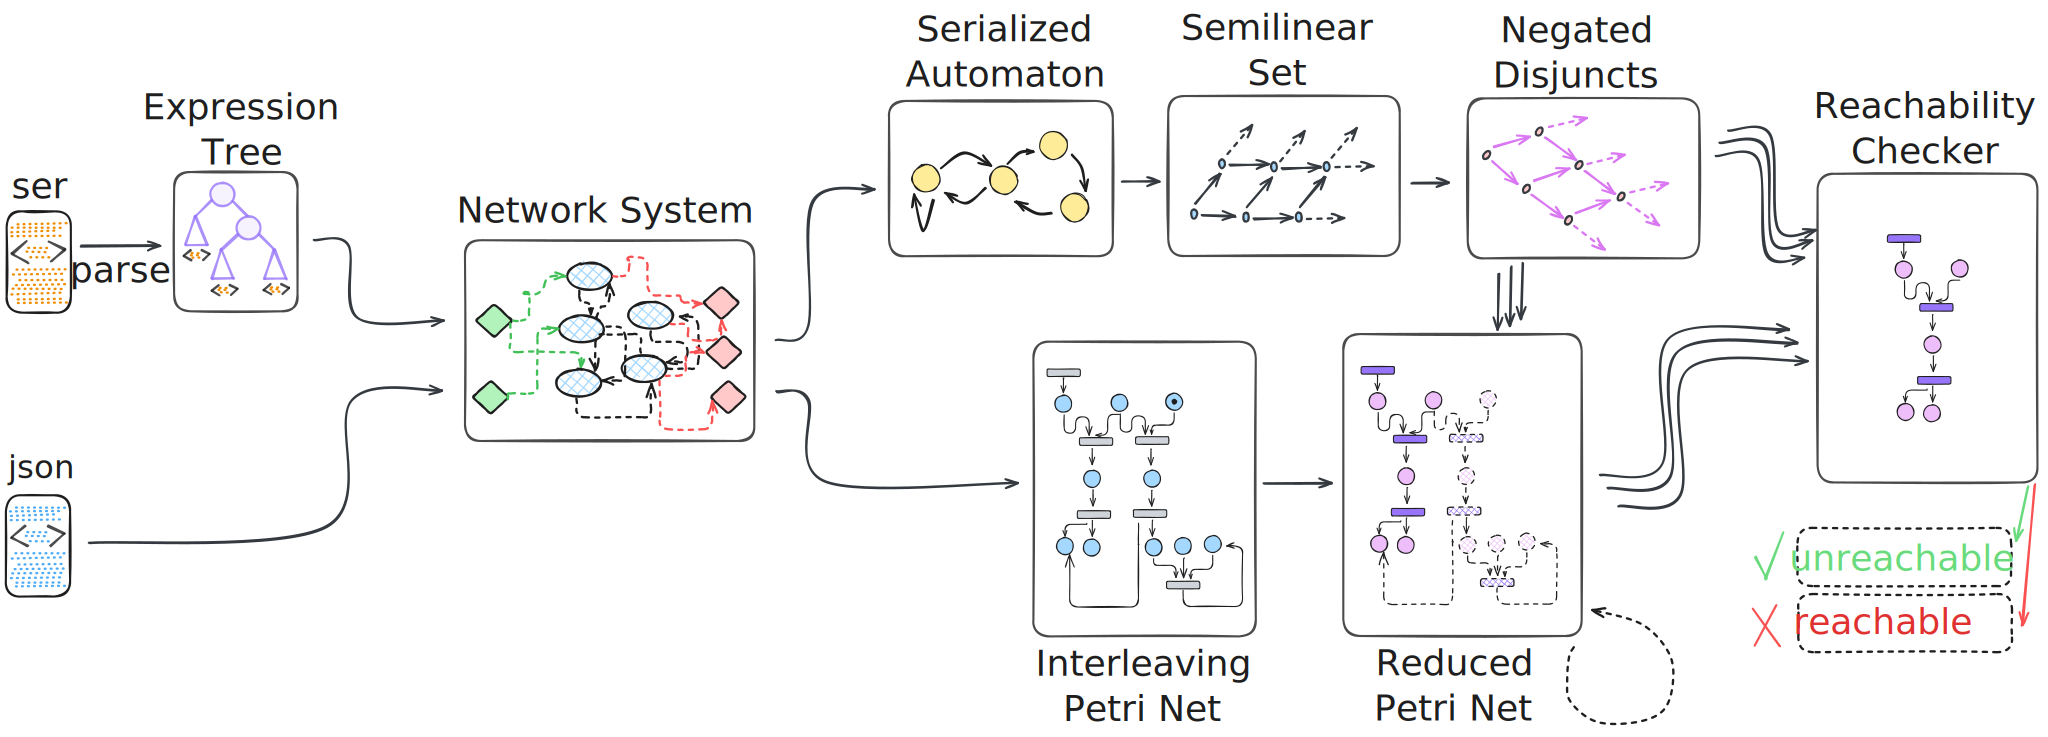
\includegraphics[width=1.0\textwidth]{plots/full_program_flow.pdf}
	\caption{Full program flow 
%		If the target set is unreachable --- a serializability proof is produced; otherwise, if it is reachable --- a counterexample trace is generated.
	(simplified, without backward arrows 
%	translating invariants (if serializable) or counterexample traces (if non-serializable) back 
	to the NS level).}
	\label{fig:full_program_flow}
\end{figure}


%\subsection{Optimizations}

%\paragraph{Bidirectional Pruning of the Petri Net}
%Before any heavy symbolic reasoning takes place, we apply bidirectional pruning on the underlying PN.  In the forward pass, we traverse from the initial marking to identify all places and transitions that could ever fire; in the backward pass, we traverse backward from any place that can influence a target constraint, and identify transitions and places that cannot contribute to reaching it.  By iteratively repeating forward passes and backward passes until convergence, we remove every component of the net that cannot both originate and contribute to the reachable target set.  This dramatically shrinks the net in practice, often converting an intractably large model into one small enough for exhaustive analysis.
%%
%We depict this in Fig.~\ref{fig:bidirectional_pruning}, and give a formal proof of correctness in Appendix~\ref{appendix:BidirectionalProof}.

%\paragraph{Redundant‐Constraint Elimination}
%When manipulating Presburger sets or their semilinear representations, it is common for some inequalities or disjuncts to add no new coverage beyond what other constraints already guarantee.  The redundant‐constraint elimination pass inspects each linear inequality and each disjunct in a disjunctive normal form, testing whether it is implied by the rest.  Any constraint or disjunct found redundant is dropped, ensuring that subsequent intersection, union, and projection operations work on the smallest necessary formula.  This streamlines the logic formula and prevents exponential blow‐up of case distinctions during solver invocations.
%
%Every time you build or star a semilinear set, you prune out any “period” vectors that are rendered useless by earlier steps:. nce you’ve accumulated a bunch of LinearSet components, you try to merge any that mathematically subsume one another:

%\paragraph{Generating Fewer Constraints}
%During set‐construction--- especially when introducing new existentially‐quantified variables or combining transition effects, we selectively avoid generating any marking that would strictly dominate an already‐seen solution.  In effect, whenever a candidate disjunct would yield a superset of an existing one, it is skipped entirely.  This ``generate‐less” heuristic stops the proliferation of large, overlapping regions in the semilinear description, trading off completeness of intermediate case‐enumeration for concise final representations.  In benchmarks with large state‐spaces, it can reduce the number of intermediate branches by orders of magnitude.

%in both the Regex and SemilinearSet Kleene-algebra instances. Concretely, instead of always building the full new structure and pruning it later, operations like union (plus) and concatenation (times) do a quick check for trivial cases and drop “zero” or “one” elements on the spo

%\paragraph{Executing Kleene Elimination in a Strategic Order:}
%When converting an NFA to a single regex, we pick the next state to eliminate by heuristically choosing the  state with the fewest incoming and outgoing edges.
%This optimization allows circumventing 
%overblown expressions resulting in naive translations, especially with regard to  Kleene closures (the “\(\mathsf{*}\)” operator).  Instead, we analyze the structure of sub-expressions under the various operators --- estimating their branching factor, and reorder them so that simpler, low‐branching components are expanded first.  This adaptive ordering often leads to early detection of fixed points or dead‐ends, preventing the combinatorial explosion that arises when complex loops are expanded prematurely.  




\subsection{Benchmark Overview} 
\label{subsec:benchmarks}
To the best of our knowledge, ours is the first and only tool to: (i) statically check serializability on \textit{unbounded} programs; and (ii) \textit{prove serializability holds}.
%
Thus, due to a lack of standard benchmarks for evaluating serializability, we 
assembled a suite of dozens of benchmarks (as part of our accompanying artifact~\cite{ArtifactRepository}).
These include both serializable and non-serializable instances encoded in both \texttt{SER} and \texttt{JSON} formats, and covering a broad range of features, including arithmetic, locks, loops, non-determinism, and more (see an overview of all our benchmarks in Table~\ref{tab:benchmarks-all} of Appendix~\ref{appendix:full_results}).
%
We note that although the benchmarks themselves are not the main part of the paper, we believe that they have merit on their own, due to their relevance to various real-world systems of interest.
%
Specifically, we wish to note our suite of benchmarks encoding \textit{network \& system protocols} (see Table~\ref{tab:networking-benchmarks}), which include stateful firewalls, BGP routing programs, network monitors, and more --- 
%highlighting the serializability challenges inherent in real-world distributed programs.
%
%Here, we were motivated by 
as motivated by real-world concurrency problems in this domain. One such example is our \textit{routing-cycle benchmark} in software-defined networks (motivated by~\cite{NaGhSa24}). Another real-world example is our \textit{snapshot isolation benchmark} (see Appendix~\ref{appendix:tour}), that was motivated by a real database bug, namely, duplicate-key errors~\cite{cockroach-issue-14099} in the popular \texttt{CockroachDB} system~\cite{cockroachdb-si-docs}.
%
In both cases and others, the non-serializable behavior was automatically identified by our toolchain.
%
%Our benchmarks include both serializable and non-serializable instances, and their features and categorization appears in Table~\ref{tab:benchmarks-all}. 



%As there are no standard benchmarks for evaluating serializability, we wrote dozens of programs in our abstract NS language. These benchmarks span a wide range of complexity --- covering branching, looping constructs, arithmetic, non-deterministic choice, and multi-request workflows that manipulate both shared (global) variables and per-request (local) state. 
%
%We include both serializable and non-serializable instances and summarize the benchmarks' features and categorizations in Table~\ref{tab:benchmarks-all}. 
%
%In particular, our most sophisticated examples are drawn from realistic networking and system-protocol scenarios, including stateful firewalls, BGP routing, network monitoring, and more --- highlighting the serializability challenges inherent in real-world distributed programs.
%
%As there are no official benchmarks for evaluating serializability, we hand-coded dozes of programs in our abstract network-system language.
%%
%The benchmarks vary in the complexity, and have multiple features: branching, loops, arithmetic, non-determinism, and multiple requests and responses, operating on both shared (global) variables and per-request (local) variables.
%%
%The benchmarks include both serializable and non-serializable instances, as we summarize in Table.~\ref{tab:benchmarks-all}, based on a category and feature-wise breakdown.
%%
%Especially, we wish to note the final category of complex examples as motivated by real-world systems and networking programs.
%%
%These include a stateful firewall, BGP routing, network monitoring and additional examples.
%
%\begin{itemize}
%		
%	\item \todo{update benchmark overview and category names}
%	\item \textbf{Core expressions \& multi request workflows}: Benchmarks testing arithmetic, boolean, and simple control expression.
%	\item \textbf{Fred (mixed arithmetic)}: Mixed control and arithmetic transformations (Fred series).
%	\item \textbf{Stop (circular-increment) series}: Circular increment loops and variants.
%	\item \textbf{Concurrency \& locking loops}: Concurrent looping patterns with locking and tricky interactions.
%	\item \textbf{Non-deterministic choice \& randomness}: Random choice and non-deterministic branching benchmarks.
%	\item \textbf{Networking \& system protocols}: Networking protocols and system-level monitoring.
%	\item \textbf{JSON state-machine examples}: Example JSON-encoded state machine workflows.
%\end{itemize}
%
%
%
%The benchmarks differ in their complexity and in the various features pertaining to them --- branching, loops, randomness, multiple requests, etc. 
%



\newpage
	This is placeholder text for implementation details.
	
	\section{Evaluation}
	% \section{Evaluation}
\label{sec:evaluation}

%\begin{enumerate}
%    \item Benchmarks (describe our benchmarks)
%    \item Results (total time, split out SMPT time from our rust code time)
%    \item Analysis of optimizations (how much time they save, petri net sizes, semilinear set sizes)
%    \item Limitations (examples we cannot solve, future work that would help)
%\end{enumerate}


\noindent
\textbf{Experimental Setup.}
All experiments ran on a Lenovo ThinkPad P16s, with 16 AMD cores and 64 GB of RAM, running on a Linux Ubuntu 24.04.2 operating system.
%
%We plan on making all our code, benchmarks raw results publicly available with the final version of this paper.
%
Our code, benchmarks, and full experimental results are publicly available~\cite{ArtifactRepository}.
%
%All experiments were run with a \texttt{TIMEOUT} value of $150$ seconds.
 



\subsection{Runtime Results}
We ran \toolname{} on all 47 benchmarks, out of which 27 are serializable, and the remaining 20 are non-serializable. 
For each benchmark, we measured the time for deciding the reachability query, as well as the overall time, including validation of the invariant proof (if serializable) or of the counterexample (if not serializable). These experiments ran in parallel on $16$ cores with all four optimizations and a \texttt{TIMEOUT} threshold of $500$ seconds.
%
Within the time limit, \toolname{} solved 26 of the 27 serializable benchmarks and 19 of the 20 non-serializable benchmarks (see summary in Table~\ref{tab:stats-summary} and the full results in Table~\ref{tab:benchmarks-all} of the appendix).
%
% As can be seen by our results (summarized in Table~\ref{tab:benchmarks-all}), withing this time limit, our tool fully solved 26/27 serializable benchmarks 
%and 19/20 non serializable benchmarks. 
%
The \textit{median} total runtime was $2{,}080$ ms across all benchmarks, and $2{,}238.50$ ms ($830$ ms) when focusing on solely serializable (non-serializable) benchmarks.
%, as reported in Table~\ref{tab:stats-summary}.
%
The \textit{average} total runtime was $52{,}857.55$ ms across all benchmarks, and $25{,}530.69$ ms ($42{,}980.47$ ms) when focusing on solely serializable (non-serializable) benchmarks.
%
We also observe a clear runtime split based on serializability: 
%For serializable benchmarks, certificate validation takes much longer than proof generation. 
among non-serializable benchmarks, counterexample generation is much longer than validation, and dominates the runtime; whereas the opposite holds in non-serializable benchmarks. This is not surprising, as validating a given counterexample only requires a polynomial-time simulation of the network to confirm its feasibility.
%
%We also note that when analyzing the benchmarks based on their serializability, there is a clear difference in their average runtime --- while in the serializable benchmarks the validation of the certificate takes significantly longer than generating the certificate (i.e., the proof) --- in the non serializable benchmarks this trend is reversed, with the overall time being dominated by the generation of the counterexample. This of course is not surprising, as counterexample generation can be done in polynomial time by emulating our network system and checking that the final counterexample can indeed be attained.
%
%We report the full results in Table~\ref{tab:stats-summary} and Table~\ref{tab:benchmarks-all}.
%, and elaborate on the per-benchmark results in Table~\ref{tab:benchmarks-all}.


%\begin{table}[!htbp]
%	\centering
%	% Load the tabular from the external file:
%	\begin{table}[H]
	\centering
	\begin{tabular}{l r r r r}
		\toprule
		& \multicolumn{2}{c}{Average time (ms)} 
		& \multicolumn{2}{c}{Median time (ms)} \\
		\cmidrule(lr){2-3} \cmidrule(lr){4-5}
		Category
		& \shortstack{certificate\\generation}
		& total
		& \shortstack{certificate\\generation}
		& total \\
		\midrule
		Serializable      &   2{,}273 &  25{,}531 &  1{,}178 &  2{,}238 \\
		Not serializable  &  42{,}076 &  42{,}980 &   773 &   830 \\
		All               &  39{,}613 &  52{,}858 &   797 &  2{,}080 \\
		\bottomrule
	\end{tabular}
\end{table}

%	\caption{Average and median runtime. Values are rounded to the nearest integer, to reduce clutter. The \textit{total} column also includes the time for validation.}
%	\label{tab:stats-summary}
%\end{table}



%\begin{table}[H]
%	\centering
%	% Load the tabular from the external file:
%	\begin{table}[H]
	\centering
	\begin{tabular}{lrrrrrr}
		\toprule
		& \multicolumn{3}{c}{Average time (ms)} & \multicolumn{3}{c}{Median time (ms)} \\
		\cmidrule(lr){2-4} \cmidrule(lr){5-7}
		Category
		& \shortstack{certificate\\generation}
		& \shortstack{certificate\\validation}
		& total
		& \shortstack{certificate\\generation}
		& \shortstack{certificate\\validation}
		& total \\
		\midrule
		Serializable      &   2273 &  23257 &  25531 &  1178 &  1300 &  2238 \\
		Not serializable  &  42076 &    905 &  42980 &   773 &    78 &   830 \\
		All               &  39613 &  13244 &  52858 &   797 &   151 &  2080 \\
		\bottomrule
	\end{tabular}
\end{table}
%\caption{Average and median runtime. Values are rounded to the nearest integer, to reduce clutter.}
%\label{tab:stats-summary}
%\end{table}





%=== Overall ===
%Certificate running time:
%Average = 39613.23
%Median  = 797.00
%
%Certificate validation time:
%Average = 13244.32
%Median  = 151.00
%
%Total running time:
%Average = 52857.55
%Median  = 2080.00
%
%=== Serializable Only ===
%Certificate running time:
%Average = 2273.38
%Median  = 1178.00
%
%Certificate validation time:
%Average = 23257.31
%Median  = 1299.50
%
%Total running time:
%Average = 25530.69
%Median  = 2238.50
%
%=== Non-Serializable Only ===
%Certificate running time:
%Average = 42075.84
%Median  = 773.00
%
%Certificate validation time:
%Average = 904.63
%Median  = 78.00
%
%Total running time:
%Average = 42980.47
%Median  = 830.00
%
%=== Percentiles (Overall) ===
%Certificate running time percentiles:
%25th percentile = 553.50
%50th percentile = 797.00
%100th percentile = 502810.00
%
%Certificate validation time percentiles:
%25th percentile = 66.50
%50th percentile = 151.00
%100th percentile = 282370.00
%
%Total running time percentiles:
%25th percentile = 615.00
%50th percentile = 2080.00
%100th percentile = 503336.00
%
%=== Percentiles (Serializable) ===
%Certificate running time percentiles:
%25th percentile = 312.00
%50th percentile = 1178.00
%100th percentile = 9858.00
%
%Certificate validation time percentiles:
%25th percentile = 115.75
%50th percentile = 1299.50
%100th percentile = 282370.00
%
%Total running time percentiles:
%25th percentile = 456.50
%50th percentile = 2238.50
%100th percentile = 292228.00
%
%=== Percentiles (Non-Serializable) ===
%Certificate running time percentiles:
%25th percentile = 628.50
%50th percentile = 773.00
%100th percentile = 356195.00
%
%Certificate validation time percentiles:
%25th percentile = 50.00
%50th percentile = 78.00
%100th percentile = 15227.00
%
%Total running time percentiles:
%25th percentile = 707.00
%50th percentile = 830.00
%100th percentile = 356299.00





\begin{table}[htbp]
	\centering
	% Load the tabular from the external file:
	\begin{table}[H] 
	\centering
	\small
	% increase horizontal padding between columns
	\setlength{\tabcolsep}{5pt}
	\renewcommand{\arraystretch}{0.9}
	\begin{tabular*}{\textwidth}{@{\extracolsep{\fill}}%
			p{2cm}     % Benchmark
			c          % Serializable
			c c c c c c % Features
			r r        % Cert, Total
		}
		\toprule
		\textbf{Benchmark}
		& \textbf{Serializable}
		& \multicolumn{6}{c}{\textbf{Features}}
		& \multicolumn{2}{c}{\textbf{Runtime (ms)}} \\
		\cmidrule(lr){1-1} \cmidrule(lr){2-2} \cmidrule(lr){3-8} \cmidrule(lr){9-10}
		& 
		& If & While & \texttt{?} & Arith & Yield & Multi-req
		& Cert. & Total \\
		\midrule
		\texttt{banking (1)}          & \xmark      & \cmark & \cmark &        & \cmark & \cmark & \cmark & 59{,}312 & 74{,}539 \\
		\texttt{banking (2)}          & \greencmark & \cmark & \cmark &        & \cmark & \cmark & \cmark & \texttt{TIMEOUT} & \texttt{TIMEOUT} \\
		\texttt{routing (1)}      & \xmark      & \cmark & \cmark & \cmark & \cmark & \cmark & \cmark & 20{,}557 & 20{,}954 \\
		\texttt{monitor (1)}       & \xmark      & \cmark & \cmark & \cmark & \cmark & \cmark & \cmark & 6{,}859  & 7{,}047 \\
		\texttt{monitor (2)}       & \greencmark & \cmark & \cmark & \cmark & \cmark & \cmark & \cmark & 3{,}047  & 12{,}324 \\
		\texttt{firewall (1)}& \xmark      & \cmark &        & \cmark & \cmark & \cmark &       & 8{,}193  & 8{,}285 \\
		\texttt{firewall (2)}& \greencmark & \cmark &        & \cmark & \cmark &       &       & 6{,}886  & 252{,}752 \\
		\midrule
		\bottomrule
	\end{tabular*}
\end{table}

	\caption{Overview of benchmarks from the network and system protocols category. 
%	For our full benchmarks see Appendix~\ref{appendix:full_results}.
}
\label{tab:networking-benchmarks}
\end{table}


\subsection{Optimization Analysis}
\label{subsec:optimization-results}

%Next of our four optimizations, and analyzed their effect on the overall runtime and space resources.
%
%All experiments were run with a \texttt{TIMEOUT} value of $150$ seconds.


\subsubsection{Runtime Optimization.}

We ran all benchmarks with each of the following six optimization combinations: 
(i) without any optimization (marked [\texttt{\textbf{\text{-}\text{-}\text{-}\text{-}}}] in Fig.~\ref{fig:timeout_cumulative_solved_log}); (ii) with bidirectional pruning (marked [\texttt{\textbf{\text{B}\text{-}\text{-}\text{-}}}]); (iii) with redundant constraint elimination (marked [\texttt{\textbf{\text{-}\text{R}\text{-}\text{-}}}]); (iv) with generation of fewer constraints (marked [\texttt{\textbf{\text{-}\text{-}\text{G}\text{-}}}]);
(v) with strategic Kleene elimination (marked [\texttt{\textbf{\text{-}\text{-}\text{-}\text{S}}}]);
and finally, (vi) with all optimizations altogether (marked [\texttt{\textbf{\text{B}\text{R}\text{G}\text{S}}}]).
%
The results of the aggregated runtimes are presented in Fig.~\ref{fig:timeout_cumulative_solved_log} and show that over $19\%$ more benchmarks are solved when using all optimizations compared to running without any optimization.
%
Not surprisingly, the best configuration is the one with all optimizations on. 
%
We also note that the best single-optimization configurations with regard to runtime are [\texttt{\textbf{\text{-}\text{-}\text{G}\text{-}}}] and [\texttt{\textbf{\text{B}\text{-}\text{-}\text{-}}}], solving over $74\%$ and $72\%$ of the benchmarks respectively. 
%
We also note that the two remaining optimizations, [\texttt{\textbf{\text{-}\text{R}\text{-}\text{-}}}] and [\texttt{\textbf{\text{-}\text{-}\text{-}\text{S}}}], performed slightly worse (although not significantly) than without the optimizations when counting overall timeouts.
%
However, when comparing the combinations, it seems that there are instances in which each of these optimizations still \textit{strictly} improves runtime.
%
For example, there are instances (see \texttt{a3.ser} and \texttt{a7.ser} in Appendix~\ref{appendix:full_results}), in which the use of the redundant constraint optimization (  [\texttt{\textbf{\text{-}\text{R}\text{-}\text{-}}}])
affords a speedup of between $72.2\%$ and $85.2\%$ over the same benchmarks without this optimization.

\subsubsection{Space Optimization.}
Our optimizations also reduce the space complexity of the two main components --- the Petri net and the semilinear set.

\noindent
(1) \textbf{Petri net.} Bidirectional pruning (Fig.~\ref{fig:petri_size_reduction}) 
eliminates the average number of places \textit{by roughly half} --- from $23.91$ down to $12.79$. This optimization proved even more effective on transitions, \textit{eliminating about two-thirds}: from $37.3$ down to $12.61$. 
%Note that the pre-pruning averages were computed over $47$ nets (one per benchmark), whereas the post-pruning averages span $224$ nets, since each pre-pruning net gives rise to a separate pruned net per each disjunct.  
%\\

\noindent
(2) \textbf{Semilinear sets.} We ran an ablation experiment in which we compared all optimizations against runs where each of the three semilinear optimizations (excluding pruning) was disabled. The redundant-constraint elimination and the fewer-constraint generation \textit{drastically} reduced component counts, with the latter being especially effective in reducing the \textit{maximal} number of components to be up to $\mathbf{931\times}$ smaller, and the \textit{average} number of components to be up to $\mathbf{223\times}$ smaller (Table~\ref{tab:semilinear-size-reduction}), when compared to the baseline executions configured with all optimizations on. 
%
For fairness, we measured only benchmarks completed under all configurations, excluding cases where semilinear sets exploded beyond $2^{30}$ components and timed out. Thus, our reported improvements actually \textit{understate} the true impact of these optimizations on memory. Such blowups, %especially common in state-machine benchmarks with NS loops, 
render even simple programs infeasible without these optimizations.
	
	
%\subsubsection{Space Optimization}
%
%Our optimizations also reduce the space complexity of the two main components --- the Petri Net and the semilinear set.
%
%\smallskip
%\noindent
%\textbf{Petri Net size reduction.}
%%
%With all optimizations enabled, we evaluated (Fig.~\ref{fig:petri_size_reduction}) the impact of our bidirectional pruning by comparing, across all benchmarks, the average number of places and transitions removed due to this optimization. On average, pruning reduced the number of places \textit{by roughly half} --- dropping from $23.91$ places before pruning to $12.79$ places afterward. Pruning proved even more effective on transitions, \textit{eliminating about two-thirds} of them: from $37.3$ transitions on average before pruning down to $12.61$ afterward. Note that the pre-pruning averages were computed over $47$ nets (one per benchmark), whereas the post-pruning averages span $224$ nets, since each pre-pruning net gives rise to a separate pruned net per each disjunct. 
%of our reachability query. 
%These results are summarized in Fig.~\ref{fig:petri_size_reduction}.

%When running our tool with all optimizations on, we analyzed the effect of our bidirectional pruning, This was done be counting the average number of places and transitions before and after pruning, on all benchmarks.
%%
%The pruning resulted in a reduction of about half the number of original places --- from $23.91$ places on average \textit{before} pruning to $12.79$ places on average \textit{after} pruning.
%%
%The bidirectional was even more effective in reducing the transitions, as demonstrated by a removing about two thirds of the transitions --- resulting in pruned Petri Nets with $37.30$ transitions on average \textit{before} pruning to $12.61$ transitions on average \textit{after} pruning.
%%
%We note that the averaging for the pre-pruning step was done on $47$ nets, once per each benchmark, while the averaging for the post-pruning step was done on $224$ nets, as each pre-pruning net can give rise to multiple post-pruning nets, one per each disjunct in our reachability query.
%%
%These results are presented in Fig.~\ref{fig:petri_size_reduction}.


%Number of values for 'Before' bars:          47
%Number of values for 'After' bars:           224
%Average number of places before pruning:     23.91
%Average number of places after pruning:      12.79
%Average number of transitions before pruning: 37.30
%Average number of transitions after pruning:  12.61






%\smallskip
%\noindent
%\textbf{Semilinear set size reduction.}
%%
%Finally, our last experiment batch analyzed the size reduction among the semilinear sets.
%%
%Towards this end, we ran all our benchmarks with all optimizations to serve as a baseline. 
%%
%Then, we analyzed the effect of the three semilinear-related optimizations, i.e., all but the bidirectional pruning. For each of these three optimizations, we ran the benchmarks with all optimizations \textit{except} the one checked.
%%
%%Table~\ref{tab:semilinear-size-reduction} include a summary of the results, when comparing the semilinear set size.
%%
%Specifically, we compare both the average and the maximal (i) number of components; and (ii) period vectors per each component, as summarized in Table~\ref{tab:semilinear-size-reduction}.
%%
%The redundant constraint elimination and the generate-less-constraints optimizations had a highly significant effect on the number of components, with the latter being especially effective in reducing the maximal number of components to be $931$ times more compact, as well as the average number of components to be $223$ times more compact, when compared to the baseline.
%%
%To ensure a fair comparison, we only measured benchmarks that were completed under every configuration, deliberately excluding any case where the optimized semilinear set exploded beyond $2^{30}$ components and timed out. By excluding these intractable runs, our reported performance improvements actually \textit{understate} the true impact of these optimizations. This explosive growth and the resulting timeouts are especially pervasive among our state-machine benchmarks due to loops in their NS, rendering even simple programs infeasible without optimizations.
%
%In fact, for both these optimizations are even more effective as, in order to conduct a fair comparison, we analyzed only benchmarks that terminated in all combinations, an hence we do not include cases in which these two optimizations rendered the original semilinear set intractable, due to having over $2^{30}$ components (!), hence timing-out and being excluded from the analysis.
%%
%This occurs pervasively in our state-machine benchmarks which have loops in their network systems --- and hence even simple programs of this category cannot be analyzed with respect to serializability.

%\todo{understand why this is related to loops in the NS}


\begin{center}
	\begin{minipage}[htbp]{0.48\textwidth}
		\centering
		\includegraphics[width=\linewidth]{figures/cactus_plot.pdf}
		\captionof{figure}{Solved instances (\texttt{T.O.} $500$ sec).}
		\label{fig:timeout_cumulative_solved_log}
	\end{minipage}\hfill
	\begin{minipage}[htbp]{0.48\textwidth}
		\centering
		\includegraphics[width=\linewidth]{figures/petri_size_reduction_plot.pdf}
		\captionof{figure}{PN size reduction via pruning.}
			%(timeout 150 seconds)
			%.}
		\label{fig:petri_size_reduction}
	\end{minipage}
\end{center}

\begin{table}[!htbp]
	\centering
	\begin{minipage}[t]{0.48\linewidth}
	\centering
	\begin{table}[H]
	\centering
	\begin{tabular}{l r r r r}
		\toprule
		& \multicolumn{2}{c}{Average (ms)} 
		& \multicolumn{2}{c}{Median (ms)} \\
		\cmidrule(lr){2-3} \cmidrule(lr){4-5}
		Category
		& \shortstack{cert.}
		& total
		& \shortstack{cert.}
		& total \\
		\midrule
		\textcolor{ForestGreen}{Serializable}      &   2{,}273 &  25{,}531 &  1{,}178 &  2{,}238 \\
		\textcolor{red}{Not serializable}  &  42{,}076 &  42{,}980 &   773 &   830 \\
		All               &  39{,}613 &  52{,}858 &   797 &  2{,}080 \\
		\bottomrule
	\end{tabular}
\end{table}

	\caption{Average and median runtime for generating certificates and the total time (also with validation).}
	%			Values are rounded to the nearest integer, to reduce clutter. 
	%The \textit{total} column also includes the time for validation.}
	\label{tab:stats-summary}
	\end{minipage}\hfill
	\begin{minipage}[t]{0.48\linewidth}
	\centering
	\begin{table}[H]
	\centering
	\begin{tabular}{l c c c c}
		\toprule
		& \multicolumn{2}{c}{components} & \multicolumn{2}{c}{periods/component} \\
		\cmidrule(lr){2-3} \cmidrule(lr){4-5}
		& average & max & average & max \\
		\midrule
	\texttt{\text{B}\text{R}\text{G}\text{S}} & 2.91 & 22 & 1.33 & 4 \\
	\texttt{\text{B}\textcolor{red}{-}\text{G}\text{S}} & 8.79 & 194 & \textbf{1.64} & 11 \\
	\texttt{\text{B}\text{R}\textcolor{red}{-}\text{S}} & \textbf{651.41} & \textbf{20{,}484} & 1.28 & \textbf{15} \\
	\texttt{\text{B}\text{R}\text{G}\textcolor{red}{-}} & 2.91 & 22 & 1.35 & 4 \\
  \bottomrule
	\end{tabular}
\end{table}

	\caption{Semilinear set size reduction via optimizations (baseline is [\texttt{\text{B}\text{R}\text{G}\text{S}}]).}
	\label{tab:semilinear-size-reduction}
\end{minipage}
\end{table}

%\begin{table}[!htbp]
%	\centering
%	% Load the tabular from the external file:
%	\begin{table}[H]
	\centering
	\begin{tabular}{l c c c c}
		\toprule
		& \multicolumn{2}{c}{num components} & \multicolumn{2}{c}{periods per component} \\
		\cmidrule(lr){2-3} \cmidrule(lr){4-5}
		& mean & max & mean & max \\
		\midrule
	baseline (all ON) & 3.64 & 24 & 1.95 & 9 \\
	no\_remove\_redundant & 30.64 & 644 & \textbf{3.46} & \textbf{39} \\
	no\_generate\_less & \textbf{566.00} & \textbf{20{,}484} & 1.38 & 15 \\
	no\_smart\_order & 3.64 & 24 & 1.97 & 9 \\
  \bottomrule
	\end{tabular}
\end{table}

%	\caption{Semilinear set size reduction via optimizations.}
%	\label{tab:semilinear-size-reduction}
%\end{table}

%\todo{Limitations?}
%Examples we cannot solve, future work that would help

%\newpage

\vspace{-5pt}



	This is placeholder text for evaluation.
	
	\section{Related Work}
	% \input{sections/6_related_work}
	This is placeholder text for related work.
	
	\section{Discussion}
	% 

\section{Discussion}
\label{sec:discussion}

%\subsection{Conclusion}


%




%\subsection{Limitations}
%\smallskip
%\noindent
\textbf{Limitations.}
While our approach advances the state of the art in verifying unbounded serializability, several limitations remain.
First, the underlying Petri Net reachability problem has \texttt{Ackermann}-complete complexity, causing our tool to time out on some complex benchmarks. %despite optimizations.
Second, our current implementation relies on \texttt{SMPT}, which may fail to find proofs even when they exist, limiting completeness.
Third, our network system model assumes a simple request/response pattern and cannot model more complex interactions, such as streaming, callbacks, or partial responses.
%Fourth, while we can verify programs with nondeterministic choice operators, we cannot handle programs with unbounded data domains or complex data structures beyond integer variables.
These limitations suggest important directions for future research.

%\subsection{Future Work}
\smallskip
\noindent
\textbf{Future Work.}
To improve \textit{scalability}, we are developing \textit{polyhedral reductions}~\cite{AmBeDa21}, a form of structural reduction~\cite{Be87,BeLeDa20} $(N_1, m_1) \vartriangleright_E (N_2, m_2)$ where $N_2$ is a simpler Petri Net and $E$ allows reconstruction of $N_1$’s state space. This would allow verification on the reduced net, with proofs lifted back to the original.
%
We also plan to \textit{extend our framework to richer communication patterns.} Beyond the current independent-client model, stronger settings include inter-client communication ---
%or Lamport’s \textit{happens-before}~\cite{La78}, while weaker ones restrict post-response communication or allow only summaries. Addressing these 
which requires 
%decentralized or streaming certification under communication constraints, 
broadening the framework to afford distributed-system guarantees.
%\todo{old}
%
%\paragraph{Scalability.}
%
%Our evaluation shows that some benchmarks still time out.
%To improve \textit{scalability}, we are developing both theory and implementation of \textit{polyhedral reductions}~\cite{AmBeDa21} --- that are structural reductions~\cite{Be87,BeLeDa20} of the form $(N_1, m_1) \vartriangleright_E (N_2, m_2)$ where $N_2$ is a simpler Petri Net and $E$ is a formula enabling reconstruction of $N_1$'s state space from $N_2$'s. This would let us verify the reduced net and lift proofs back to the original net.
%
%\guy{Nicolas are you sure about the next sentence? Do you have an explanation or a "negative proof"?}
%
%Furthermore, we note that polyhedral reductions are the only type of structural reduction for which such a conversion is possible.
%
%We are developing both theory and implementation for this extension.
%
%\todo{Limitations?}
%Examples we cannot solve, future work that would help
%To conclude..
%
%
%
%In another axis, we aim to \textit{extend our framework to more diverse communication patterns.}
%\paragraph{Extensions to diverse communication models.}
%Currently, clients act independently: each issues a request, receives a response, then verification is centralized. Stronger models allow inter-client communication or partial orderings (Lamport’s \textit{happens-before}~\cite{La78}); weaker ones forbid post-response communication or permit only limited summaries. Addressing such settings will require decentralized certification or streaming proofs under communication constraints. Extending our framework along these axes would capture a broader class of practical distributed-system guarantees.


%\paragraph{Extensions to diverse communication models.}
%
%Our current framework assumes that clients act independently --- each submits a request, receives a response, and only afterward collaborates to verify (in a centralized manner) whether the combined outcomes are serializable. However, in a stronger model, clients may communicate during execution or enforce partial ordering of their interactions. More generally, this can be formalized via Lamport’s \textit{happens‐before} relation over request/response pairs~\cite{La78}. 
%%
%In contrast, a weaker model disallows communication --- in which case clients either cannot communicate after receiving responses or may only share limited summaries. Jointly deciding serializability in this setting will require decentralized certification techniques or streaming proofs that respect tight communication constraints. 
%%
%By extending our theory and tool along these two axes, we aim to cover a broad spectrum of practical distributed‐system guarantees, that are more complex and match broader, real-world scenarios.

%
%
%
%\todo{Different notions of serializability}
%\begin{itemize}
%    \item \todo{Current notion: clients independently submit a request and get a response, and later they all get together and see if what they got was serializable}
%    \item \todo{Stronger: clients are not independent, or sequentially execute some parts. General: we have some happens-before on the requests/responses}
%    \item \todo{Weaker: the clients cannot communicate with each other afterwards to determine whether what they got was serializable, or they can only communicate in a limited way}
%    \item \todo{Infinite / unbounded executions}
%\end{itemize}



\smallskip
\noindent
\textbf{Conclusion.}
We present the first implemented tool that verifies serializability for unbounded concurrent systems and generates proof certificates.
Our approach bridges theory and practice, with the following key contributions:
% by implementing Bouajjani et al.'s decision procedure with crucial optimizations that make it practical.
%
%Key contributions include: 
(1) formalizing serializability for network systems, (2) implementing the decision procedure with proof generation, (3) developing optimizations that reduce complexity by orders of magnitude, and (4) demonstrating feasibility on various benchmarks inspired by real-world systems.

	This is placeholder text for discussion.
	
	\section*{Data and Software Availability}
	The data and software are available.
	
	\section*{Acknowledgements}
	The work of Amir was partially supported by a Rothschild Fellowship.
	
	% Bibliography
	% \bibliographystyle{splncs04}
	% \bibliography{references}
	
	\newpage
	\appendix
	\section{Appendix}
	This is placeholder text for the appendix.
	
\end{document}